\documentclass{prova}

\usepackage{amsmath}
\usepackage{amsfonts}

\setlength{\textheight}{25cm}

\renewcommand{\sin}{\,\mbox{sen}\,}
\newcommand{\tg}{\,\mbox{tg}\,}
\newcommand{\ds}{\displaystyle}

\professor{Prof.\@ Adriano Barbosa}
\disciplina{C\'alculo Diferencial e Integral}
\avaliacao{P1}
\curso{Engenharia de Aquicultura}
\data{20/09/2021}

\begin{document}
	\cabecalho{5}  % o numero 5 indica a qnt de quadros na tabela de nota

    \textbf{Todas as respostas devem ser justificadas.}

    \begin{questionario}
        \q{Uma caixa deve ser construída a partir de uma folha de papelão
           retangular medindo 12cm por 10cm recortando quatro quadrados iguais
           como na figura abaixo e dobrando na linha pontilhada.}
            \begin{questionario}
                \qq{Encontre a expressão que calcula o volume da caixa em
                    função da medida do lado do quadrado que será recortado.
                    Explique detalhadamente como você chegou a essa expressão.}
                \qq{Observando as dimensões da caixa e seu volume, determine o
                    domínio da função encontrada no item anterior.}
                    
            \end{questionario}
            \begin{figure}[h]
                \centering
                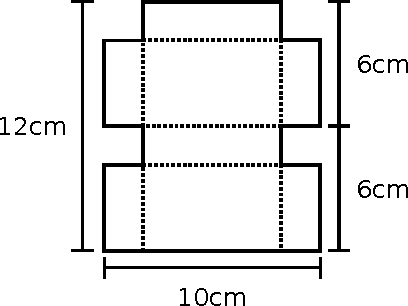
\includegraphics[width=0.3\textwidth]{caixa.pdf}
            \end{figure}
        %\q{Determine os valores de $k$ tais que o limite abaixo exista:}
        %    \[\lim_{x\rightarrow 4}\left(\frac{k}{4-x^2}-\frac{1}{1-x}\right)\]
        \q{Calcule os limites:}
            \begin{questionario}
                \qq{$\ds\lim_{x\rightarrow 16}\frac{16-x}{4-\sqrt{x}}$.}
                \qq{$\ds\lim_{x\rightarrow 3^-}\frac{x-3}{9-x^2}$.}
            \end{questionario}
        \q{Seja $f(x)=x^5-2x^4+3x^3-3x^2+2x-1$:}
            \begin{questionario}
                \qq{Calcule o limite $\ds\lim_{x\rightarrow\infty} f(x)$.}
                \qq{Calcule o limite $\ds\lim_{x\rightarrow-\infty} f(x)$.}
                \qq{Qual o maior intervalo onde $f$ é contínua?}
                \qq{Conclua que $f$ tem pelo menos uma raiz real.}
            \end{questionario}
            [Dica: reescreva $f$ colocando $x^5$ em evidência para calcular os
            limites.]
        \q{Dado $y=x\sin{x}$, calcule $y''+y$.}
        \q{Determine os valores do intervalo $\left(-\frac{\pi}{2},
           \frac{\pi}{2}\right)$ onde a reta tangente de $f(x)=\sec{(x)}$ é
           horizontal, ou seja, $f'(x)=0$.}
    \end{questionario}
\end{document}
